\documentclass[11pt]{article}
\usepackage{enumerate}
\usepackage{amsfonts}
\usepackage{graphicx}
\usepackage{listings}
\usepackage{float}
\usepackage{tikz}
\usepackage{subcaption}


\pagestyle{empty} \setlength{\parindent}{0mm}
\addtolength{\topmargin}{-0.5in} \setlength{\textheight}{9.5in}
\addtolength{\textwidth}{0.5in} \addtolength{\oddsidemargin}{-0.5in}

\begin{document}

\begin{center}
\textbf{Logan Sims \\ CSCI 402 \\ Homework 2  }
\end{center}

\begin{enumerate}[1.]
\item
  \begin{enumerate}[a.]
  \item
  The state space for this problem can be represented as a four-tuple in the following way:\\\\
  N: The set of states, a state a configuration of the game board.\\
  A: The set of arcs that represent actions taken to go from one state to the next.\\
  S: The start state.\\
  GD: The goal state.\\
  
  Actions in this state space will be represented as moving the blank, similar to the 8-puzzle example. The two legal moves now become://
  \begin{enumerate}[i.]
  \item Exchange blank with a tile to the left or right of it for a cost of one.
  \item Exchange the blank with a title 2 or 3 tiles away. This has a cost of the blank from the exchange tile minus one. 
  \end{enumerate}
  
  A Breadth-first search could be used to explore all states in this space. It would be possible for a state to be discovered multiple times causing loops. However by keeping track of open and closed states these states will not be explored again. 
  
  \item
  A heuristic for this problem could be counting the number of white tiles that are to the right of the black tiles. By counting tiles and making moves that help to decrease the number of incorrect tile placements this heuristic can find a solution. Since the goal state requires all white tiles be on the left the program would choose paths that attempt to get closer to the goal state.\\
  
  Using the approach to determine admissibility presented in the textbook this heuristic is admissible because counting the tiles out of place is less than or equal to the number of moves required to get to the goal state.\\
  
  This heuristic is not monotonic. . \\
  
  The heuristic is more informed than a breadth-first search because it is able to prioritize paths that could lead to a goal state. Breadth-first search simple performs an unbiased exploration of the state space.\\
  \end{enumerate}

\item
  \begin{enumerate}[a.]
  \item The following 8-puzzle start state demonstrates a reversal. The solution to this puzzle requires 13 moves to solve.

\begin{figure}[htbp]
    \centering
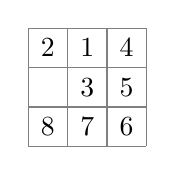
\begin{tikzpicture}
\draw[step=0.5cm,color=gray] (-1,-.5) grid (.5,1);
\node at (-0.75,+0.75) {2};
\node at (-0.25,+0.75) {1};
\node at (+0.25,+0.75) {4};

\node at (-0.75,+0.25) {};
\node at (-0.25,+0.25) {3};
\node at (+0.25,+0.25) {5};

\node at (-0.75,-0.25) {8};
\node at (-0.25,-0.25) {7};
\node at (+0.25,-0.25) {6};
\end{tikzpicture}
\end{figure}


\begin{center} 
\begin{tabular}{| l | l | l |} 
\hline Number & \textbf{Heuristic} & \textbf{Estimate}\\
\hline 1 & Tiles out of place. & 8\\ 
\hline 2 & Sum of distance out of place. &  9\\ 
\hline 3 & 2x number of direct reversals. & 4  \\ 
\hline 4 & Sum dist. out of place plus 2x num. reversals. & 13 \\
\hline 
\end{tabular} 
\end{center} 

Based on the example above the 4th heuristic is equal to the exact result making it the most accurate.\\
  \item
  Since it was established in the text that the 2nd heuristic was the most informed compared to the 1st and 3rd there only needs to be a comparison of the 2nd and 4th. Seeing as how the 4th takes into account that reversals are costly it will in fact prune the state space more efficiently that the 2nd heuristic. This makes the 4th heuristic the most informed.\\
  \item
  
  \item

  \end{enumerate}
\end{enumerate}
\end{document}